
%(BEGIN_QUESTION)
% Copyright 2006, Tony R. Kuphaldt, released under the Creative Commons Attribution License (v 1.0)
% This means you may do almost anything with this work of mine, so long as you give me proper credit

%{\it Differential} thermocouple circuits are used to measure the difference in temperature between two points:

Differansetermoelement kretser brukes for å måle termperaturforskjellem mellom to punkter. 

$$\includegraphics[width=15.5cm]{i00401x01.eps}$$

%Does the indicating instrument require reference junction compensation or not?  Explain your answer.

Trenger instrumentet i dette tilfellet et referansepunkt? Begrunn svaret. 

\underbar{file i00401}
%(END_QUESTION)





%(BEGIN_ANSWER)

No reference junction compensation is needed at the indicator, because no reference junction exists there.  In effect, the thermocouple at $T_2$ serves as a ``reference'' junction to the thermocouple at $T_1$.

A practical application for a differential thermocouple is in a solar heating system for a house.  During the day time, solar energy will ensure that the collector is at a greater temperature than the house which it warms.  At night, however, when the sun is not shining, the collector will be colder than the house.  In this state, you do {\it not} want the circulating pump (or blower) to run, for that would transfer heat out of the warm house and dissipate it through the cold collector.  A differential thermocouple could tell you (by the polarity of its voltage) which was warmer: the collector or the house.  Then, an op-amp comparator circuit could disable the circulating pump to prevent heat loss through the collector at night.

%(END_ANSWER)





%(BEGIN_NOTES)


%INDEX% Measurement, temperature: differential thermocouples

%(END_NOTES)


